\section{Artur Sojka}
\label{sec:artsoj}

A diagram showing Lagrange points in the Sun-Earth system (see Figure~\ref{fig:points}).

\begin{figure}[htbp]
    \centering
    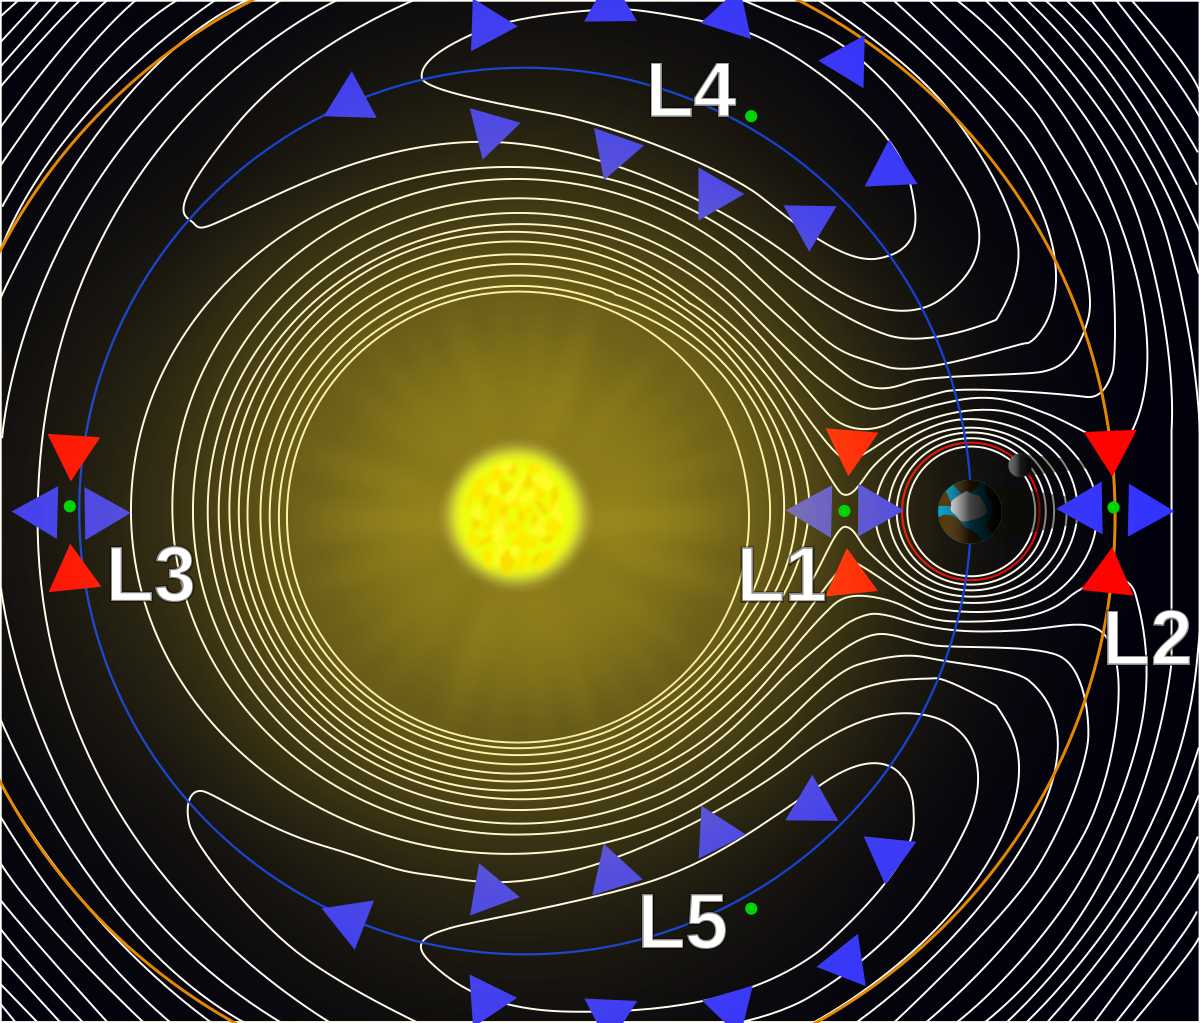
\includegraphics[width=0.6\textwidth]{pictures/Lagrange_points.png}
    \caption{Sun-Earth Lagrange points}
    \label{fig:points}
\end{figure}

Table ~\ref{tab:stability} Represents stability of Lagrange points.

\begin{table}[htbp]
\centering
\begin{tabular}{|c|c|}
 \hline
 {} & \textbf{STABILITY} \\ [0.5ex]
 \hline
 \textbf{L1} & UNSTABLE \\
 \hline
 \textbf{L2} & UNSTABLE \\
 \hline
 \textbf{L3} & UNSTABLE \\
 \hline
 \textbf{L4} & STABLE \\
 \hline
 \textbf{L5} & STABLE \\
 \hline
\end{tabular}
\label{tab:stability}
\end{table}

Here is the equation for the force of gravity. \[F=G\frac{m_1m_2}{r^2}\]

A regular list
\begin{itemize}
    \item One
    \item Two
    \item Three
    \begin{itemize}
        \item Three and a half
    \end{itemize}
\end{itemize}

\begin{samepage}
An enumerated list.
\begin{enumerate}
    \item First
    \item Second
    \item Third
\end{enumerate}
\end{samepage}
\vspace{0.5cm}
In celestial mechanics, the Lagrange points (also \textbf{Lagrangian points} or \textbf{libration points}) are points of equilibrium for small-mass objects under the influence of two massive orbiting bodies. Mathematically, this involves the solution of the restricted \emph{three-body problem} in which two bodies are far more massive than the third.

Normally, the two massive bodies exert an \underline{unbalanced} gravitational force at a point, altering the orbit of whatever is at that point. At the Lagrange points, the gravitational forces of the two large bodies and the centrifugal force \underline{balance} each other. This can make Lagrange points an excellent location for satellites, as few orbit corrections are needed to maintain the desired orbit. 

\textbf{Normally, the two massive bodies exert an \underline{unbalanced} gravitational force at a point, altering the orbit of whatever is at that point. At the Lagrange points, the gravitational forces of the two large bodies and the centrifugal force \underline{balance} each other. This can make Lagrange points an excellent location for satellites, as few orbit corrections are needed to maintain the desired orbit.}
